\section{83 - MAT - WS 4.1, AN 1.2, AN 1.3, WS 1.3, WS 1.2 - Wachstumskurve von Kindern - Matura NT 1 16/17}

\begin{langesbeispiel} \item[6] %PUNKTE DES BEISPIELS

Um die Entwicklung der Körperhöhe und der Masse eines Kinder kontrollieren zu können, sind im Mutter-Kind-Pass die Perzentielenkurven für Körperhöhen (Größe) und Masse angegeben (Körperhöhe in cm, Masse in kg). Perzentile teilen die Körperhöhen und Massen der Kinder in Prozent-Bereiche auf. Liegt ein Wert auf dem 10. Wachstumsperzentil, so sind 10\,\% der Kinder des ausgewählten Alters kleiner oder gleich dem angegebenen Wert und 90\,\% größer oder gleich dem angegebenen Wert.

Es ist üblich, alle Werte zwischen dem 3. und dem 97. Perzentil als "`normal"' zu bezeichnen. Das folgende Diagramm zeigt die Wachstums- und Körpermassekurven für Buben im Alter von 0 bis 18 Jahren:

\begin{center}
\resizebox{0.8\linewidth}{!}{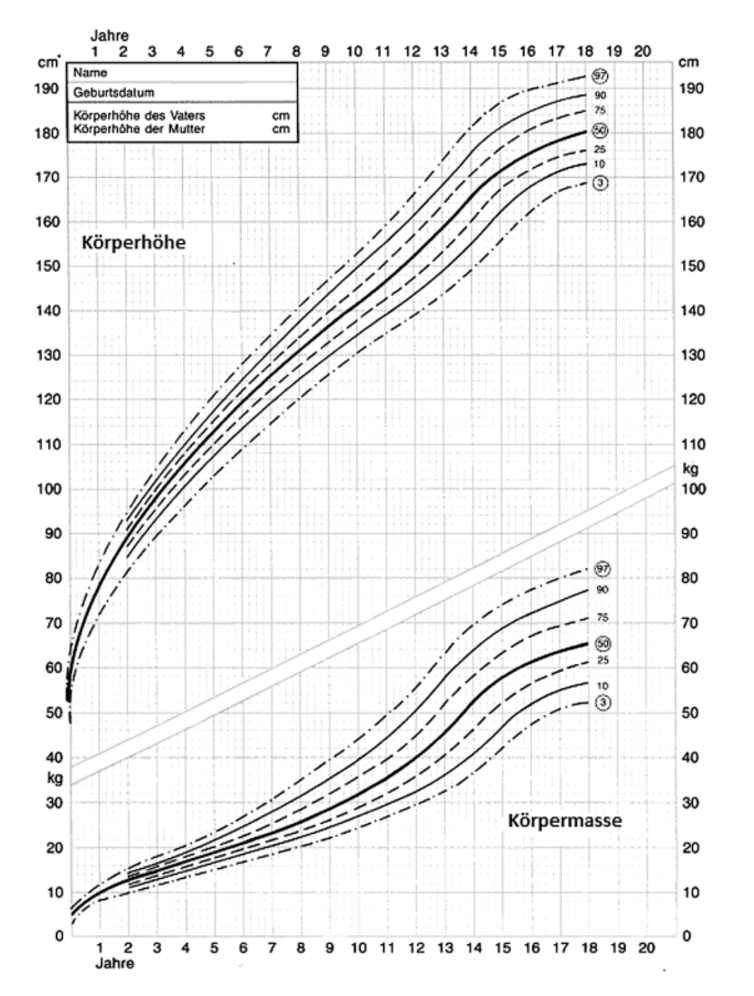
\includegraphics{../Bilder/Bild83-1.eps}}
\end{center}

\subsection{Aufgabenstellung:}
\begin{enumerate}
	\item Ein Schularzt untersucht eine zufällige Stichprobe von 8-jährigen Buben aus seinem Schulbezirk und erhebt unter anderem deren Körpermassen (in kg). Anhand der Ergebnisse dieser Messung erstellt er für den Anteil der 8-jährigen Buben aus einem Schulbezirk, deren Körpermasse im "`Normalbereich"' $[20\,\text{kg};35\,\text{kg}]$ liegt, das symmetrische Konfidenzintervall $[0,8535;0,9465]$ mit dem Konfidenzniveau $\gamma=0,95$.\leer
	
	Gib den Unterschied des der Berechnung zugrundeliegenden Stichprobenanteils zum Anteil der 8-jährigen Buben mit einer Körpermasse im "`Normalbereich"' laut Diagramm in Prozentpunkten an!\leer
	
	Berechne die Anzahl der bei dieser Stichprobe gemessenen 8-jährigen Buben!\leer
	
	\item Angenommen, für ein bestimmtes Kind sind die Körperhöhen $g(1),g(2),g(3),...$ zum ersten, zweiten, dritten usw. Geburtstag bekannt.
	
	Gib verbal oder als Formel an, wie sich die durchschnittliche Wachstumsgeschwindigkeit dieses Kindes in dem dreijährigen Zeitraum zwischen dem 6. und dem 9. Geburtstag bestimmen lässt.\leer
	
	Betrache das Größenwachstum auf dem 50. Perzentil nach dem 8. Lebenjahr. Gib das ungefähre Alter von Buben an, bei dem deren momentane Wachstumsgeschwindigkeit am größten ist!\leer
	
	\item Gib an, welcher statistischen Kennzahl derjenige Wert entspricht, den man auf dem 50. Perzentil ablesen kann.\leer
	
	Erläutere, welche Schwierigkeiten auftreten, wenn man aus dem angegebenen Diagramm ein Kastenschaubild (Boxplot) zur Darstellung der Körperhöhen von 8-jährigen Buben erstellen möchte!
	
	\end{enumerate}

\antwort{
\begin{enumerate}
	\item \subsection{Lösungserwartung:} 

Stichprobenanteil: 0,9

Anteil laut Diagramm: 0,94

Unterschied: 4 Prozentpunkte\leer

Mögliche Berechnung:

$0,9465=0,9+1,96\cdot\sqrt{\dfrac{0,9\cdot (1-0,9)}{n}}\Rightarrow\approx 160$ Buben
\subsection{Lösungsschlüssel:}
\begin{itemize}
	\item Ein Punkt für die richtige Lösung.
	\item Ein Punkt für die richtige Lösung.
	
	Toleranzintervall: $[155\text{ Buben};165\text{ Buben}]$
	
	Die Aufgabe ist auch dann als richtig gelöst zu werten, wenn bei korrektem Ansatz das Ergebnis aufgrund eines Rechenfehlers nicht richtig ist.
\end{itemize}

	\item \subsection{Lösungserwartung:}

Die durchschnittliche Wachstumsgeschwindigkeit in diesem Zeitraum entspricht einem Drittel der Größenzunahme.

oder:

$\frac{g(9)-g(6)}{3}$\leer

Das ungefähre Alter von Buben, bei dem deren momentane Wachstumsgeschwindigkeit am größten ist, liegt bei ca. 13 Jahren.

\subsection{Lösungsschlüssel:}
\begin{itemize}
	\item Ein Punkt für eine (sinngemäß) korrekte Antwort bzw. eine richtige Formel. Äquivalente Formeln sind als richtig zu werten.	
	\item Ein Punkt für die richtige Lösung, wobei die Einheit "`Jahre"' nicht angeführt sein muss.
	
	Toleranzintervall: $[12\text{ Jahre};14\text{ Jahre}]$
\end{itemize}

\item \subsection{Lösungserwartung:}

Die statistische Kennzahl, die demjenigen Wert entspricht, den man auf dem 50. Perzentil ablesen kann, ist der Median.

Die Schwierigkeiten bestehen darin, dass man zwar das 1. und das 3. Quartil sowie den Median, jedoch weder Minimum noch Maximum ablesen kann (und auch keine Informationen bezüglich Ausreißern hat).

\subsection{Lösungsschlüssel:}
\begin{itemize}
	\item Ein Ausgleichspunkt für das Anführen der korrekten statistischen Kennzahl.
	\item Ein Punkt für eine (sinngemäß) korrekte Erläuterung.
\end{itemize}
\end{enumerate}}
		\end{langesbeispiel}